\documentclass{article}
\usepackage{listings}
\usepackage{blindtext}
\usepackage[utf8]{inputenc}
\usepackage{graphicx}
\usepackage{verbatim}

\graphicspath{ {./img/} }

\title{Algorithmen und Datenstrukturen: Lösungsbuch Aufgabe 1}
\author{Frederik Dudzik}
\date{\today}

\begin{document}
\maketitle

\section{Implementation}
\subsection{Main}
In Main werden die Daten initialisiert und das Programm immer wieder von vorne ausgeführt bis der Nutzer das Programm schließt.
Die Eingabe der Befehle erfolgt hier, jedoch werden die Befehle in einer anderen Prozedur interpretiert und ausgeführt.
Das Ziel dahinter ist, dass das Programm einfacher zu verstehen ist, da wir die Verantwortung teilen und hinter weniger abstrakten Prozeduren bündeln.

\subsection{CLI}
Die CLI Prozeduren dienen als ein Adapter zwischen der eigentlichen Logik des Programms und der Außenwelt.
Über die Funktion \texttt{cli\_function} werden die Befehle des Nutzers Interpretiert und die jeweilige adapter Funktion in cli.c aufgerufen.
Diese Funktionen gehen sicher dass die fur den gegebenen Befehls notwendigen Prozeduren ausgeführt werden.
Und das diese mit korrekten Daten verwendet werden.

\subsection{util}
In der util Datei sind hilfreiche Funktionen gespeichert die in keine der anderen Dateien platz finden und auch keiner eigenen Datei bedürfen.
Wenn dies ein größeres Projekt wäre hätte ich die Funktionen in eigene Dateien ausgelagert.
Da sonst solch eine util Datei ein schwarzes Funktions-Loch fur Entwickler werden würde.

\subsection{student}
In student.c sind alle Funktionen implementiert die die Student Struktur betreffen.
Das interessanteste in der Datei ist wie ich das Subject Enum definiere.
Wir brauchen in dem Code die Subjects einmal als Enum und als String.
Dafür benutzte ich den Preprozessor damit ich die Subjects nicht zweimal hinschreiben muss und damit sie in der gleichen Reihenfolge sind.

\subsection{\texttt{cli\_student}}
In \texttt{cli\_student} sind adapter Prozeduren für Student. Siehe die Sektion CLI.

\subsection{\texttt{student\_list}, doppelt und einfach}
Das Interface für die Doppelt wie einfach Verkettete Liste ist bei mir die selbe, weswegen sie sich eine header Datei teilen.
Diese wird von den anderen Dateien included.
Damit wir angeben welche Listenform wir verwenden wollen müssen wir beim Kompilieren oder im Code \texttt{DOUBLE\_LINKED\_LIST} definieren oder undefiniert lassen.
Daraufhin wird die jeweilige Listenstruktur und implementation von \texttt{student\_list.h} kompiliert.

\subsection{Makefile}
Das Makefile ist weitestgehend aus den Unterlagen übernommen.
Ich habe dieses lediglich fur meine Bedürfnisse erweitert.

Wichtig ist das sie mit `make` die einfache \texttt{student\_list} kompilieren und mit \texttt{\'make double\'} die doppelte. 

\subsection{TODO}
Das Pattern das in Main und CLI beschrieben wurde sollte strikter durchgezogen werden.
Z.b. sollte in den Prozeduren von \texttt{cli\_student} nicht direkt einen Studenten erzeugt werde, die cli Funktionen sollte das erledigen.
Zudem sollte die Liste als eine generische Implementiert werden, falls das Programm geschrieben werden würde.
Ausserdem sollten man mehr mit Status Codes arbeiten. In der CLI wird versucht das zu implementieren. Dies ist jedoch eher dürftig umgesetzt worden.

\section{Aufgabe 3}    
\subsection{b: zum Hinzuf{\"u}gen eines Elements vor dem ersten Element}
Wir müssen keine Verbindung zu vorherigen Element setzten.
Dadurch sparen wir 6 Operationen.

\subsection{a: Erstellen eines neuen Elements}
Wir müssen keine Verbindung zu vorherigen Element setzten.
Dadurch sparen wir 4 Operationen.

\subsection{g: L{\"o}schen eines Elements.}
Wir müssen keine Verbindung zu vorherigen Element setzten.
Dadurch sparen wir 2 Operationen.

\subsection{c: Hinzuf{\"u}gen eines Elements nach dem letzten Element}
Wir müssen die Liste einmal durchlaufen um ein Element am Ende hinzuzufügen O(n).
Bei einer Doppeltverketteten Liste ist es O(1), da wir über den end Listenkopf direkt darauf zugreifen können.

\section{Aufgabe 5}

\subsection{ Meine Implementierung }

\begin{comment}
\begin{lstlisting}

void swapStudents(StudentList* prev, StudentList* next)
{
    Student* tmp = prev->student;  //2
    prev->student = next->student; //3
    next->student = tmp;                 //2
}


\end{lstlisting}
\end{comment}

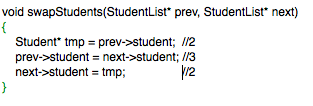
\includegraphics{swapstudents}

O(7)
\begin{comment}
\begin{lstlisting}

//selectionsort
void sortMatrikel(StudentList* sl)
{
    StudentList* j   = 0L;                                  		//1
    StudentList* min = 0L;                                  		//1
    StudentList* i   = sl;                                  		//1
    while(i->next->next != 0L) {					//3 		-------|
        i   =i->next;                                       			//1			|
        min = i;                                            			//1			|
        j   = i;                                            			//1         		|
        while (j->student != 0L){                           		//2 	----|    	| 
            if (j->student->id < min->student->id) min = j; //4/w/5   |     	|
            j = j->next;                                    			//2	     |n   	| n
        }                                                   			//  	----|     	|
        if(min != i) swapStudents(min, i);			//7               	|
    }                                                      			// 		-------|
}

\end{lstlisting}
\end{comment}

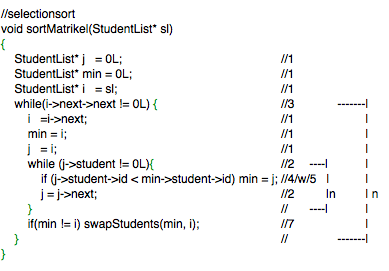
\includegraphics{selectionsort}

$1+1+1+n*(3+1+1+1+n*(2+5+2+7)) \Rightarrow  n*n = O(n^2)$

$1+1+1+n*(3+1+1+1+n*(2+4+2+7)) \Rightarrow  n*n = \Omega(n^2)$

\begin{comment}
\begin{lstlisting}

//bubblesort
void sortStudiengang(StudentList* sl)
{
    StudentList* i = sl;                                          				//1
    int swapped = false;                                           			//1
    do {                                                         					/w/ ----------------|
        swapped = false;                                           			//1        	        |
        while (i->next->next->student != 0L) {                    		//4  	-------|       |
            i=i->next;                                            				//2    		|       |
            if (i->student->subject > i->next->student->subject) {	//6        	|       |
                swapStudents(i, i->next);                         			/w/8   	| n    | n
                swapped = true;                                    			/w/9		|       |
            }                                                     					// 		|       |
        }                                                         					//   	-------|       |
        i = sl;                                                   				//1         	        |
    } while (swapped);                                             			// 	--------------|
}

\end{lstlisting}
\end{comment}

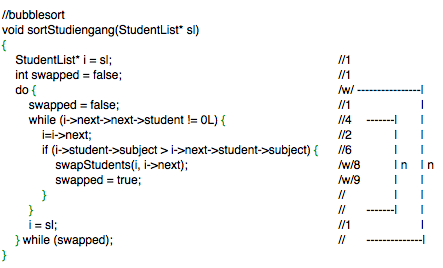
\includegraphics{bubblesort}

$1+1+n*(1+4+n*(2+6+8+9)+1 \Rightarrow  n*n = O(n^2)$

$1+1+(1+4+n*(2+6)+1        \Rightarrow  n   = \Omega(n)$

\newpage
\subsection{Allgemein}
Bubblesort ist aus "Algorithmen und Datenstrukturen" Auflage 5 von Thomas Ottmann und Peter Widmayer entnommen. 
Sellectionsort ist aus Donald Knuth's 'The Art of Computer Programming, Volume 3: Sorting and Searching'

\begin{comment}
\begin{lstlisting}[mathescape]

//Bubblesort
procedure bubblesort(var a: sequence);
  var i: integer;                                			 //  1
  begin                                         
    repeat                                        			/w/ -----------|
      for i:=1 to (N-1) do                        		//	---|	  |
        if a[i].key > a[i+1].key                  		//  6	    | n	  | n
          then {vertausche a[i] und a[i+1]}       	/w/ 4 ---|	  |
    until {keine Vertauschungen mehr auftreten}  //  ------------|
  end

\end{lstlisting}
\end{comment}

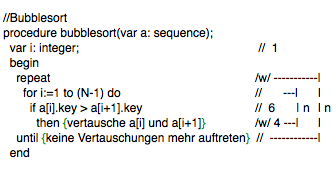
\includegraphics{bubblesortallgemein}

$1+n*(n*(6+4) \Rightarrow n*n = O(n^2)$

$1+n*(6)     \Rightarrow  n   = \Omega(n)$
\newpage

\begin{comment}
\begin{lstlisting}

//Selectionsort
int i,j;					//2
int iMin;				//1 
for (j = 0; j < n-1; j++) {	//3  ---------|
    iMin = j;				//1             |
    for ( i = j+1; i < n; i++) {	//3 -----|     |
        if (a[i] < a[iMin]) {       //1       |     |
            iMin = i;                  /w/1    | n  | n
        }                                 //         |     |
    }                                     //  ------|     |
    if(iMin != j) {                   //1             |
        swap(a[j], a[iMin]);     /w/3	         | 
    }                                     //               |
}                                         //    ---------|

\end{lstlisting}
\end{comment}

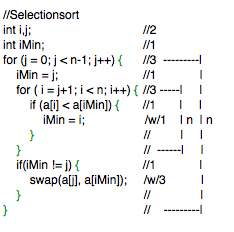
\includegraphics{selectionsortallgemein}

$2+1+3+n*(1+3+n*(1+1)+1+3) \Rightarrow  n*n = O(n^2)$

$12+1+3+n*(1+3+n*(1)+1)    \Rightarrow  n   = \Omega(n)$

\subsection{Ergebnis}

Die Komplexität von meiner Implementierung unterscheidet sich nicht von der Allgemeinen.

\subsection{Begründung der Auswahl}
Die Algorithmen können genauso in einer einfach wie doppelt verketteten Liste implementiert werden ohne einen Komplexität Verlust zu erleiden. Im Gegensatz zu Insertion sort zum Beispiel.
Ich habe eine einfachere Implementation vorgezogen, anstatt einer schnelleren.

\end{document}
